% Baccalauréat malgache, série C, 2005 : corrigé partiel.
\TCDBacAttribution{C}{2005}
\TCDPartial{Corrigé partiel : il s’arrête à la question 2(b) de la partie A du problème II ; la suite de la partie A et la partie B ne sont pas corrigées.}
\providecommand{\Milimetre}[2]{%
									\clip #1 rectangle #2;
									\draw [xstep=0.1cm,ystep=0.1cm,opacity=.05,line width=.05] #1 grid #2;
									\draw [xstep=0.5cm,ystep=0.5cm,opacity=0.1,line width=0.1] #1 grid #2;
									\draw [xstep=1.0cm,ystep=1.0cm,opacity=0.2,line width=0.2] #1 grid #2;
									}

\providecommand{\dx}{~\mathrm{d}x}
\providecommand{\Re}[1]{\mathrm{Re}\left( #1 \right)}
\providecommand{\Im}[1]{\mathrm{Im}\left( #1 \right)}
\providecommand{\dt}{\mathrm{d}t}
\providecommand{\Ouv}{(O;\vec{u},\vec{v})}
\providecommand{\mes}[2]{\mathrm{mes}\left( \widehat{ \overrightarrow{#1} ; \overrightarrow{#2} } \right)}
\providecommand{\D}{(\mathscr{D})}
\providecommand{\Courbe}{(\mathscr{C})}
\providecommand{\Courben}{(\mathscr{C}_n)}
\providecommand{\CourbeU}{(\mathscr{C}_1)}
\providecommand{\CourbeD}{(\mathscr{C}_2)}
\providecommand{\bary}[1]{\mathrm{bar}\left\lbrace #1 \right\rbrace}
\providecommand{\CourbeT}{(\mathscr{C}_3)}
\providecommand{\congru}[3]{#1 \equi #2 \quad \left[ \mathrm{mod}~#3\right]}
\providecommand{\Angl}[2]{\left( \widehat{ \overrightarrow{#1} , \overrightarrow{#2} } \right)}
%
%%%%%%%%%%%%%%%%%%%%%%%%%%%%%%%%%%%%%%%%%%%%%%%%%%%%%%%%%%%%%%%%%%%%%%%%%%%%%%%%%%%%%%%%%%%%%%%%%%%%%%%%%%%%%%%%%%%%%%%%%%%%%%%%
\noindent \underline{\textsc{\textbf{Exercice}}} (4 points) 
	\begin{enumerate}
		\item 
			\begin{enumerate}
				\item \vln{Solution particuli\`ere de \eqref{eq:Bac C 2005 Arithm 1} :}
						Comme $2 \cdot 1 - 1 = 1$ alors \ansbox{$(1,1)$} est une solution particuli\`ere.
				\item \vln{R\'esolution de \eqref{eq:Bac C 2005 Arithm 1}}
						R\'esolvons d'abord l'\'equation $2x_h - y_h = 0$.
						On a $2x_h = y_h$ donc $2 | y_h$. Ainsi, $y_h = 2k$ et $2 x_h = 2 k \Rightarrow x_h = k$, $k \in \mathbb{Z}$.
						
						On a alors 
						\[
							\left.
								\begin{array}{r}
									2 x_h 	- y_h 	= 0 \\
									2 x_0 - y_0 = 1 
								\end{array}
							\right\rbrace
							\Rightarrow
							2 (x_h + x_0) - (y_h + y_0) = 1 .
						\]
						Donc l'ensemble des solutions est 
						\ansbox{$\displaystyle{ \{ (k + 1 , 2k + 1) \mid k \in \mathbb{Z} \} }$}.
			\end{enumerate}
		\item \vln{Relation qui lie $a$ et $b$ :}
				L'\'ecriture binaire de $A$ donne $b + 6 = A = 2^2 + 2 a + 1$.
				Donc $b + 6 = 5 + 2a$, ce qui entra\^ine \ansbox{$2a - b = 1$}.
		\item \vln{R\'esolution du syst\`eme :}
				Comme $PGCD(x,y) = 12$, il existe $(k,\ell)$ tel que $x = 12 k $ et $y = 12 \ell$.
				De plus, $PGCD(k,\ell) = 1$.
				Comme $x + y = 60$ on a $12 k + 12 \ell = 60$ ou encore $k + \ell = 5$ et $PGCD(k,\ell) = 1$.
				Les possibilit\'es pour $(k,\ell)$ sont : $(1,4)$, $(2,3)$, $(3,2)$ et $(4,1)$.
				Les valeurs de $(x,y)$ correspondantes sont : \ansbox{$(12,48)$, $(24,36)$, $(36,24)$ et $(48,12)$}.
		\item 
			\begin{enumerate}
				\item \vln{Calcul des probabilit\'es de $A$ et $B$ :}
					Notons d'abord que pour $U_1$, le nombre de tirages possible est $6$ tandis que
					pour $U_2$, le nombre de tirages possibles est $\Comb{6}{2} = 15$.
					\begin{description}
						\item[$P(A) = $] 
							$
									\left( \frac{2}{6} \times \frac{\Comb{2}{2}}{\Comb{6}{2}} \right)
									+ \left( \frac{3}{6} \times \frac{\Comb{3}{2}}{\Comb{6}{2}} \right) 
						=	\left(\frac{1}{3} \cdot \frac{1}{15}\right)
									+ \left( \frac{1}{2} \cdot \frac{3}{15} \right)
								=	\frac{1}{45} + \frac{1}{10}
							$
							ce qui donne \ansbox{$P(A) = \frac{11}{90}$}.
						\item[$B$ :]
							$ (1,\{1,2\}) $ ou $ (2,\{0,2\}) $ ou $ (2,\{1,1\}) $.
							Ainsi, 
							$
								P(B)	=		\left(\frac{3}{6} \times \frac{\Comb{3}{1} \cdot \Comb{1}{1}}{\Comb{6}{2}}\right)
											+	\left(\frac{1}{6} \times \frac{\Comb{2}{1} \cdot \Comb{1}{1}}{\Comb{6}{2}}\right)
											+	\left(\frac{1}{6} \times \frac{\Comb{3}{2}}{\Comb{6}{2}}\right)
										=		\left(\frac{1}{2} \times \frac{3}{15}\right)
											+	\left(\frac{1}{6} \times \frac{2}{15}\right)
											+	\left(\frac{1}{6} \times \frac{3}{15}\right)
										=		\frac{1}{10} + \frac{1}{45} + \frac{1}{30}
							$
							ce qui donne \ansbox{$P(B) = \frac{7}{45}$}.
					\end{description}
				\item \vln{Probabilit\'e de $C$ :}
					Analysons d'abord les solutions de l'\'equation $2 x - y = 1$ :
					\begin{description}
						\item[Si $x = 0$,] $y = -1$ ce qui est impossible dans notre cas.
						\item[Si $x = 1$,] $y = 1$ ce qui correspond \`a $0 + 1$.
						\item[Si $x = 2$,] $y = 3$ ce qui correspond \`a $1 + 2$.
					\end{description}
					Ainsi, 
					$P(C)	=	\left(\frac{3}{6}\times\frac{\Comb{2}{1}\cdot\Comb{3}{1}}{\Comb{6}{2}}\right)
								+\left(\frac{1}{6}\times\frac{\Comb{3}{1}\cdot\Comb{1}{1}}{\Comb{6}{2}}\right)
							=	\left(\frac{1}{2} \cdot \frac{6}{15}\right)
								+\left(\frac{1}{6} \cdot \frac{3}{15}\right)
							=	\frac{1}{5} + \frac{1}{30}
						$
					ce qui donne \ansbox{$P(C) = \frac{7}{30}$}.
			\end{enumerate}
	\end{enumerate}
%%%%%%%%%%%%%%%%%%%%%%%%%%%%%%%%%%%%%%%%%%%%%%%%%%%%%%%%%%%%%%%%%%%%%%%%%%%%%%%%%%%%%%%%%%%%%%%%%%%%%%%%%%%%%%%%%%%%%%%%%%%%%%%%
\noindent \underline{\textsc{\textbf{PROBLEME I}}} (7 points) \newline
	\textbf{Partie 1}\\[-1\baselineskip]
		\begin{enumerate}
			\item \label{qest: Bac C 2005 Pbm I Part I, 1/}
				\begin{enumerate}
					\item \label{qest: Bac C 2005 Pbm I Part I, 1/ a)}
						\vln{Montrons que $\overrightarrow{JI} = \frac{\overrightarrow{JA}+\overrightarrow{JB}}{2}$
											et $\overrightarrow{JK} = \frac{\overrightarrow{JA}+\overrightarrow{JC}}{2}$}
							Notons d'abord que $I$ est milieu de $[AB]$ signifie que 
							$\overrightarrow{IA} + \overrightarrow{IB} = \vec{0}$.
							Comme la relation de Chasles donne 
							\[
								\left.
									\begin{array}{r}
										\overrightarrow{JA} = \overrightarrow{JI} + \overrightarrow{IA}	\\
										\overrightarrow{JB} = \overrightarrow{JI} + \overrightarrow{IB}
									\end{array}
								\right\rbrace
								\Rightarrow
								\overrightarrow{JA} + \overrightarrow{JB} 
									= 2 \overrightarrow{JI} + \underbrace{\overrightarrow{IA} + \overrightarrow{IB}}_{\vec{0}}
							\]
							alors \ansbox{$\frac{\overrightarrow{JA}+\overrightarrow{JB}}{2} = \overrightarrow{JI}$}.
							
							De m\^eme, $K$ est milieu de $[AC]$ signifie que 
							$\overrightarrow{KA} + \overrightarrow{KC} = \vec{0}$.
							Comme la relation de Chasles donne 
							\[
								\left.
									\begin{array}{r}
										\overrightarrow{JA} = \overrightarrow{JK} + \overrightarrow{KA}	\\
										\overrightarrow{JC} = \overrightarrow{JK} + \overrightarrow{KC}
									\end{array}
								\right\rbrace
								\Rightarrow
								\overrightarrow{JA} + \overrightarrow{JC} 
									= 2 \overrightarrow{JK} + \underbrace{\overrightarrow{KA} + \overrightarrow{KC}}_{\vec{0}}
							\]
							alors \ansbox{$\frac{\overrightarrow{JA}+\overrightarrow{JC}}{2} = \overrightarrow{JK}$}.

						\vln{D\'eduisons que $\overrightarrow{IK} = \frac{1}{2} \overrightarrow{BC}$}
							Commen\c{c}ons par remarquer que 
							$\overrightarrow{IJ} = - \overrightarrow{JI} = - \frac{\overrightarrow{JA}+\overrightarrow{JB}}{2}
							= \frac{-\overrightarrow{JA}-\overrightarrow{JB}}{2} = \frac{\overrightarrow{AJ}+\overrightarrow{BJ}}{2}$.
							On a alors 
							\[
								\overrightarrow{IK} = \overrightarrow{IJ} + \overrightarrow{JK}
									= \frac{\overrightarrow{AJ}+\overrightarrow{BJ}}{2} + \frac{\overrightarrow{JA}+\overrightarrow{JC}}{2}
									= \frac{
										\overrightarrow{AJ}+\overrightarrow{JA}
										+\overrightarrow{BJ}+\overrightarrow{JC}}{2}
									= \frac{1}{2} \overrightarrow{BC} .
							\]

					\item 
						\vln{Montrons que $\overrightarrow{KI} = \frac{\overrightarrow{KA}+\overrightarrow{KB}}{2}$
											et $\overrightarrow{KJ} = \frac{\overrightarrow{KB}+\overrightarrow{KC}}{2}$}
							Notons $I$ est milieu de $[AB]$ signifie que 
							$\overrightarrow{IA} + \overrightarrow{IB} = \vec{0}$.
							La relation de Chasles donne 
							\[
								\left.
									\begin{array}{r}
										\overrightarrow{KA} = \overrightarrow{KI} + \overrightarrow{IA}	\\
										\overrightarrow{KB} = \overrightarrow{KI} + \overrightarrow{IB}
									\end{array}
								\right\rbrace
								\Rightarrow
								\overrightarrow{KA} + \overrightarrow{KB} 
									= 2 \overrightarrow{KI} + \underbrace{\overrightarrow{IA} + \overrightarrow{IB}}_{\vec{0}}
							\]
							alors \ansbox{$\frac{\overrightarrow{KA}+\overrightarrow{KB}}{2} = \overrightarrow{KI}$}.
							
							De m\^eme, $J$ est milieu de $[BC]$ signifie que 
							$\overrightarrow{JB} + \overrightarrow{JC} = \vec{0}$.
							La relation de Chasles donne 
							\[
								\left.
									\begin{array}{r}
										\overrightarrow{KB} = \overrightarrow{KJ} + \overrightarrow{JB}	\\
										\overrightarrow{KC} = \overrightarrow{KJ} + \overrightarrow{JC}
									\end{array}
								\right\rbrace
								\Rightarrow
								\overrightarrow{KB} + \overrightarrow{KC} 
									= 2 \overrightarrow{KJ} + \underbrace{\overrightarrow{JB} + \overrightarrow{JC}}_{\vec{0}}
							\]
							alors \ansbox{$\frac{\overrightarrow{KB}+\overrightarrow{KC}}{2} = \overrightarrow{KJ}$}.

						\vln{D\'eduisons que $\overrightarrow{IJ} = \frac{1}{2} \overrightarrow{AC}$}
							Commen\c{c}ons par remarquer que 
							$\overrightarrow{IK} = - \overrightarrow{KI} = - \frac{\overrightarrow{KA}+\overrightarrow{KB}}{2}
							= \frac{-\overrightarrow{KA}-\overrightarrow{KB}}{2} = \frac{\overrightarrow{AK}+\overrightarrow{BK}}{2}$.
							On a alors 
							\begin{align*}
								\overrightarrow{IJ}
									&= \overrightarrow{IK} + \overrightarrow{KJ}\\
									&= \frac{\overrightarrow{AK}+\overrightarrow{BK}}{2}
									 + \frac{\overrightarrow{KB}+\overrightarrow{KC}}{2}\\
									&= \frac{
										\overrightarrow{AK}+\overrightarrow{KC}
										+\overrightarrow{BK}+\overrightarrow{KB}}{2}
									 = \frac{1}{2}\overrightarrow{AC}.
							\end{align*}
					\item \vln{Montrons que $(AIJK)$ est un carr\'e}
						D'une part,
						$\overrightarrow{IJ} = \frac{1}{2} \overrightarrow{AC} = \overrightarrow{AK}$
						donc $AIJK$ est un parall\'elogramme.
						
						D'autre part $\mes{AI}{AK} = \mes{AB}{AC} = \frac{\pi}{2}$
						donc $AIJK$ est un rectangle (parall\'elogramme ayant un angle droit).
						
						De plus, $AI = \frac{1}{2} AB = 2\cm$ et $IJ = AK = \frac{1}{2} AC = 2\cm$
						donc $AIJK$ poss\`ede trois c\^ot\'es de m\^eme mesures.
						
						On d\'eduit que \ansbox{$AIJK$ est un carr\'e}.
						
						\vln{Figure}
						\begin{figure}[H]
						\centering
							\begin{tikzpicture}[line cap=round,line join=round,>=triangle 45,x=1.0cm,y=1.0cm]
								\draw (0,0) -- (4,0) -- (0,4) -- cycle;
								\draw[dashed] (0,0)-- (4,4);
								\draw (0,0)-- (4,0);
								\draw (4,0)-- (0,4);
								\draw (0,4)-- (0,0);
								\draw (2,0)-- (2,2);
								\draw (0,2)-- (2,2);
								\begin{scriptsize}
									\fill [color=black] (0,0) circle (1.5pt) node[above left] {$A$};
									\fill [color=black] (4,0) circle (1.5pt) node[above right] {$B$};
									\fill [color=black] (0,4) circle (1.5pt) node[below left] {$C$};
									\fill [color=black] (2,0) circle (1.5pt) node[below] {$I$};
									\fill [color=black] (2,2) circle (1.5pt) node[above] {$J$};
									\fill [color=black] (0,2) circle (1.5pt) node[left] {$K$};
									\fill [color=black] (4,4) circle (1.5pt) node[below] {$E$};
								\end{scriptsize}
							\end{tikzpicture}
						\end{figure}
				\end{enumerate}
			\item 
				\begin{enumerate}
					\item \vln{Image de $I$ par $t$}
						D'apr\`es la question~\ref{qest: Bac C 2005 Pbm I Part I, 1/}~\ref{qest: Bac C 2005 Pbm I Part I, 1/ a)} :
						$\overrightarrow{IK} = \frac{1}{2} \overrightarrow{BC}$,
						ce qui montre que \ansbox{$t(I) = K$}.
						
						\vln{Image de $K$ par $r$}
							$AIJK$ \'etant un carr\'e :
							\[
								\left.	
									\begin{tabular}{r}
										JK = JI	\\
										$\mes{JK}{JI} = \frac{\pi}{2}$
									\end{tabular}
								\right\rbrace
								\Rightarrow
								\ansbox{$r(K) = I$}.
							\]
					\item \vln{Image de $I$ par $f = r \circ t$}
						On a $f(I) = r \left( t(I) \right) = r(K) = I$.
						Donc \ansbox{$f(I) = I$}.
						
						\vln{Nature et \'el\'ements caract\'eristiques de $f$}
							Comme $f$ est la compos\'ee d'une rotation d'angle $\frac{\pi}{2}$ et d'une translation 
							alors $f$ est une rotation d'angle $\frac{\pi}{2}$.
							Comme $f(I) = I$, alors $I$ est le centre de $f$.
							
							Ainsi, \ansbox{$f$ est la rotation de centre $I$ et d'angle $\frac{\pi}{2}$}.
					\item \vln{Image de $K$ par $g = t \circ r$}
						On a $g(K) = t \left( r(K) \right) = t(I) = K$.
						Donc \ansbox{$g(K) = K$}.
						
						\vln{Nature et \'el\'ements caract\'eristiques de $g$}
							Comme $g$ est la compos\'ee d'une translation et d'une rotation d'angle $\frac{\pi}{2}$
							alors $g$ est une rotation d'angle $\frac{\pi}{2}$.
							Comme $g(K) = K$, alors $K$ est le centre de $g$.
							
							Ainsi, \ansbox{$g$ est la rotation de centre $K$ et d'angle $\frac{\pi}{2}$}.
				\end{enumerate}
			\item \vln{Rapport et angle de $S$}
				$\displaystyle{
					\left.
						\begin{array}{r}
							S(B) = E \\
							S(J) = C
						\end{array}
					\right\rbrace
				}$
				donc 
				le rapport de $S$ est $\frac{EC}{BJ}$ et
				l'angle de $S$ est $\mes{BJ}{EC}$.
				
				Les diagonales $[AE]$ et $[BC]$ du quadrilat\`ere $ABEC$ se coupent en leur milieu $J$.
				De plus, ce quadrilat\`ere poss\`ede deux c\^ot\'es, $AB$ et $AC$, de m\^eme longueurs et formant un angle droit.
				En d\'eduit que $ABEC$ est un carr\'e.
				
				On sait alors que $2 BJ = BC = \sqrt{2} EC$ ce qui implique que $\frac{EC}{BJ} = \frac{2}{\sqrt{2}} = \sqrt{2}$.
				
				Comme $\overrightarrow{EC} = \overrightarrow{BA}$ alors $\mes{BJ}{EC} = \mes{BJ}{BA} = \frac{\pi}{4}$.
				
				Ainsi, $S$ est une similitude plane directe de
				\ansbox{rapport $\sqrt{2}$ et d'angle $\frac{\pi}{4}$}.
		\end{enumerate}

\noindent
	\textbf{Partie 2}\\[-1\baselineskip]
		\begin{enumerate}
			\item \vln{Coordonn\'ees de $E$ et $J$}
				Comme $\overrightarrow{AE} = \overrightarrow{AB} + \overrightarrow{AC} = 4 \vec{e_1} + 4 \vec{e_2}$,
				alors \ansbox{$E(4,4)$}.
				Comme $\overrightarrow{AJ} = \frac{1}{2} \overrightarrow{AE}$, alors \ansbox{$J(2,2)$}.
			\item 
				\begin{enumerate}
					\item \vln{\'Ecriture complexe de $S$}
						Pour tout point $X$, on note par $z_X$ son affixe.
						On a donc $z_A = 0$, $z_B = 4$, $z_C = 4i$, $z_J = 2 + 2i$ et $z_E = 4 + 4i$.
						
						Soit $z' = a \, z + b$ l'\'ecriture complexe de $S$.
						Comme $S(B) = E$ et $S(J) = C$, alors 
						$a = \frac{z_E - z_C}{z_B - z_J} = \frac{4 + 4 i - 4i}{4 - 2 - 2i} = \frac{4}{2 - 2i} = 1 + i$
						et
						$b = z_E - a \, z_B = 4 + 4i - (1+i) \cdot 4 = 4 + 4i - 4 - 4i = 0$.
						Ainsi, l'\'ecriture complexe de $S$ est \ansbox{$z' = (1+i) \, z$}.
					\item \vln{Coordonn\'ees du centre $\Omega$ de $S$}
						Comme $0 = (1+i) \, 0$, alors $\Omega$ a pour affixe $0$, et donc pour coordonn\'ees \ansbox{$(0,0)$}.
						Autrement dit, $\Omega$ est l'origine $A$.
				\end{enumerate}
			\item 
				\begin{enumerate}
					\item \vln{Nature et \'el\'ements caract\'eristiques de $\overline{S}$}
						Notons par $h$ l'homoth\'etie de centre $A$ et de rapport $\sqrt{2}$
							et par $r$ la rotation de centre $A$ et d'angle $\frac{\pi}{4}$.
						Soit $\Delta$ la bissectrice de l'angle $\Angl{AB}{AE}$.
						On a alors 
						\begin{align*}
							\overline{S}	& =		S \circ S_{(AB)}			&	S	& =		h \circ r							\\
											& =		h \circ r \circ S_{(AB)}	&	r	& =		S_{\Delta} \circ S_{(AB)}	\\
											& =		h \circ S_{\Delta} \circ S_{(AB)} \circ S_{(AB)}						\\
											& =		h \circ S_{\Delta}	.
						\end{align*}
							Ainsi, $\overline{S}$ est la similitude plane indirecte de centre $A$,
							de rapport $\sqrt{2}$ et d'axe $\Delta$.
					\item \vln{Ecriture complexe associ\'ee \`a $\overline{S}$}
						D\'eterminons d'abord l'\'ecriture complexe de $S_{(AB)}$ :
						puisqu'il s'agit d'une sym\'etrie axiale, son \'ecriture complexe est de la forme $z' = a \, \bar{z} + b$.
						\[
							\left.
								\begin{array}{r}
									S(A) = A \\
									S(B) = B
								\end{array}
							\right\rbrace
							\Rightarrow
							a = \frac{z_A - z_B}{\overline{(z_A - z_B)}} = \frac{-4}{-4} = 1.
						\]
						$b = z_A - a \cdot \overline{z_A} = 0 - 0 = 0$.
						Donc l'\'ecriture complexe de $S_{(AB)}$ est $z' = \bar{z}$.
						
						Comme $\overline{S} = S \circ S_{(AB)}$ alors son \'ecriture complexe est \ansbox{$z' = (1+i) \bar{z}$}.
				\end{enumerate}
		\end{enumerate}
%%%%%%%%%%%%%%%%%%%%%%%%%%%%%%%%%%%%%%%%%%%%%%%%%%%%%%%%%%%%%%%%%%%%%%%%%%%%%%%%%%%%%%%%%%%%%%%%%%%%%%%%%%%%%%%%%%%%%%%%%%%%%%%%
\noindent \underline{\textsc{\textbf{PROBLEME II}}} (9 points) \newline
%%%%%%%%%%%%%%%%%%%%%%%%%%%%%%%%%%%%%%%%%%%%%%%%%%%%%%%%%%%%%%%%%%%%%%%%%%%%%%%%%%%%%%%%%%%%%%%%%%%%%%%%%%%%%%%%%%%%%%%%%%%%%%%%
	\begin{description}
		\item[Partie A]
			\begin{enumerate}
				\item On a $g(x) = (1-x) \ln (1-x) - x$ pour tout $x \in ]-\infty ;0 [$.
					\begin{enumerate}
						\item \vln{Variation de $g$}
							On a 
							$
								g'(x)	=	(-1) \ln (1-x) + (1-x) \cdot \frac{(-1)}{1-x} - 1
										=	- \ln (1-x) - 2 .
							$
							Comme $x<0$, on a $-x>0$ et donc $1-x>1$, ce qui entra\^ine
							$\ln(1-x)>0$ et $-\ln(1-x)<0$.
							On d\'eduit alors que $g'(x)=-\ln(1-x)-2<0$ et, par cons\'equent, que $g$ est d\'ecroissante.
								
								\vln{Tableau de variation de $g$}
									\begin{align*}
										\left.
											\begin{array}{r}
												\Lim_{x\rightarrow-\infty} 1-x = +\infty			\\
												\Lim_{x\rightarrow-\infty} \ln(1-x) = +\infty
											\end{array}
										\right\rbrace
										\Rightarrow
										\Lim_{x\rightarrow-\infty} (1-x) \ln (1-x) = +\infty
									\end{align*}
									De plus, comme $\Lim_{x\rightarrow-\infty} -x = +\infty$ alors 
									$\Lim_{x\rightarrow-\infty} (1-x) \ln (1-x) - x = +\infty$.
									
									\begin{align*}
										\left.
											\begin{array}{r}
												\Lim_{x\rightarrow 0} 1-x = 1			\\
												\Lim_{x\rightarrow 0} \ln(1-x) = 0	\\
												\Lim_{x\rightarrow 0} -x = 0
											\end{array}
										\right\rbrace
										\Rightarrow
										\Lim_{x\rightarrow 0^-} (1-x) \ln (1-x) - x = 0
									\end{align*}
									
									On a alors le tableau de variation de $g$ : 
									\ansbox{
										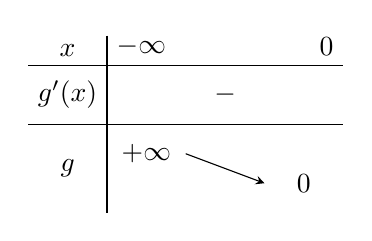
\begin{tikzpicture}[>=stealth,y=.75cm]
											\draw (-1,0) -- (3,0);
											\draw (-1,-1) -- (3,-1);
											\draw (0,.5) -- (0,-2.5);
											\draw (-.5,.25) node {$x$};
											\draw (0,0) node[above right] {$-\infty$};
											\draw (-.5,-.5) node {$g'(x)$};
											\draw (-.5,-1.75) node {$g$};
											\draw (3,0) node[above left] {$0$};
											\draw (1.5,-.5) node {$-$};
											\draw[->] (1,-1.5) -- (2,-2);
											\draw (.5,-1.5) node {$+\infty$};
											\draw (2.5,-2) node {$0$};
										\end{tikzpicture}
										}
						\item \vln{Signe de $g(x)$}
								Un examen du tableau de variation montre que $g(x)>0$ pour tout $x\in]-\infty;0[$.
					\end{enumerate}
				\item 
					\begin{enumerate}
						\item \vln{Montrons que $f$ est continue en $x_0 = 0$}
							\vspace{-1\baselineskip}
							\begin{align*}
								\Lim_{x\rightarrow 0^+} f(x) = \Lim_{x\rightarrow 0^+} (1-x) \, \expo{\frac{x}{2}} = 1 = f(0)
							\end{align*}
								donc $f$ est continue \`a droite en $x_0$.
							%
							\begin{align*}
								\Lim_{x\rightarrow 0^-} f(x) = \Lim_{x\rightarrow 0^-} 1 + \frac{x}{2} \ln (1-x) = 1 = f(0)
							\end{align*}
								donc $f$ est continue \`a gauche en $x_0$.
							
							On d\'eduit que $f$ est continue en $x_0$. \qed
						\item \vln{Calcul de $\Lim_{x\rightarrow 0^-} \frac{f(x) - f(0)}{x}$}
							\vspace{-1\baselineskip}
								\begin{align*}
									\Lim_{x\rightarrow 0^-} \frac{f(x) - f(0)}{x}
										&= \Lim_{x\rightarrow 0^-}
										   \frac{1 + \frac{x}{2}\ln(1-x) - 1}{x}\\
										&= \Lim_{x\rightarrow 0^-}\frac{1}{2}\ln(1-x)
										 = 0.
							\end{align*}
							Ainsi, \ansbox{$\Lim_{x\rightarrow 0^-} \frac{f(x) - f(0)}{x} = 0$}.
					\end{enumerate}
			\end{enumerate}
	\end{description}
































